\section{}
The system shown below consists of a pulley (radius $r$) pinned about point $O$, which is connected
to a uniform rod (length $L$) that is pinned about point $R$. The system is supported by two springs
$k_1$ and $k_2$, connected to points $A$ and $B$, respectively. The cable connecting the pulley and
rod can be considered approximately inextensible (ie. the pulley and rod are rigidly connected).
Assume small oscillations.

\begin{enumerate}[label=(\alph*)]
    \item (5 pts) Determine the effective stiffness of the system with respect to $\theta_2$ using
        the stiffness approach, by setting $\theta_2 = 1$.
    \item (5 pts) Assume that a downward force of 5 N is applied at the rod's centre of mass (point
        $G$) while the system is initially as shown above. Using your answer from part a), determine
        the resulting compression of spring $k_2$ if $r = 0.5$ m, $L = 3$ m, and $k_1 = k_2 = 100$
        N/m.
\end{enumerate}

\subsection*{Solution}
\subsection{}
\begin{figure}[h]
    \centering
    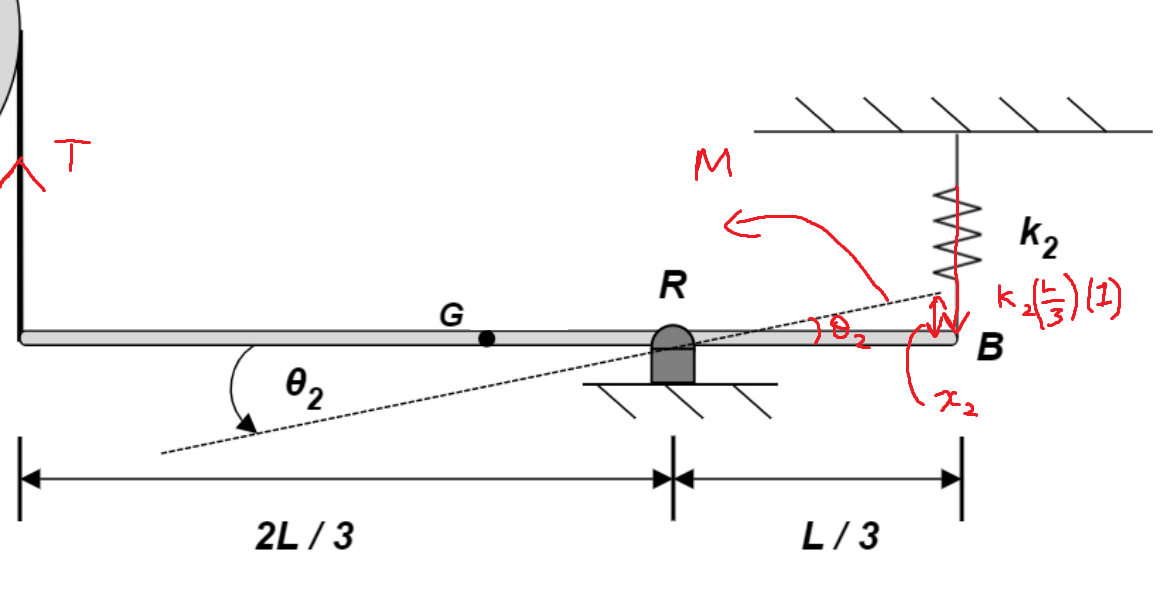
\includegraphics[width=0.5\linewidth]{Questions/Figures/q2 bar fbd.png}
    \caption{Free body diagram of the bar}
    \label{fig:q2_bar_fbd-png}
\end{figure}
\begin{figure}[h]
    \centering
    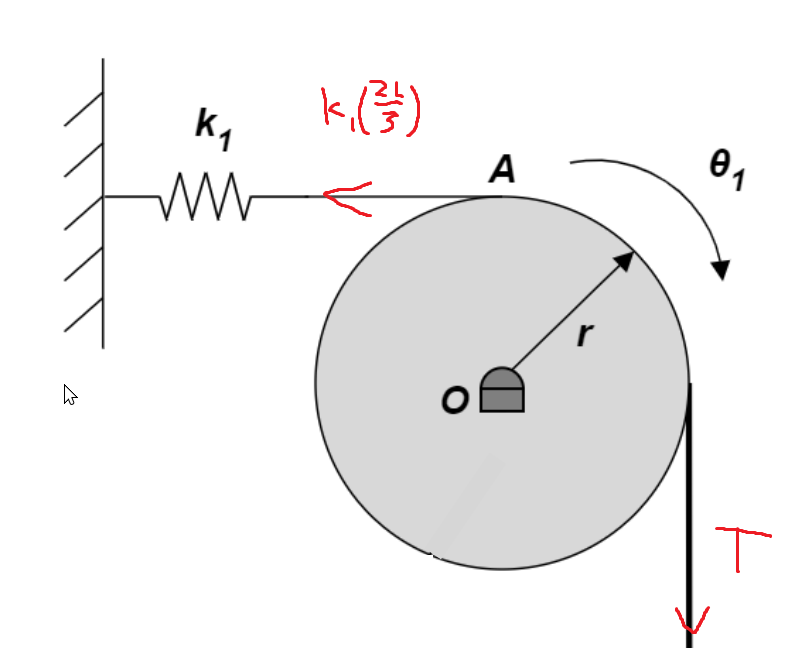
\includegraphics[width=0.5\linewidth]{Questions/Figures/q2 pulley fbd.png}
    \caption{Free body diagram of the pulley}
    \label{fig:q2_pulley_fbd-png}
\end{figure}

From the free body diagrams from the bar, we can take the sum of moment about the pivot point $R$
\begin{gather*}
    \circlearrowleft \sum M_R = 0 \\
    \implies -k_2 \left(\frac{L}{3}\right)^2 - T \left(\frac{2L}{3}\right) + M = 0 \\
    \implies M = \frac{k_2 L^2}{9} + \frac{2L}{3} T 
\end{gather*}
From the free body diagram of the pulley, we can take the sum of moments about the pivot point $O$
\begin{gather*}
    \circlearrowleft \sum M_O = 0 \\
    \implies k_1 \left(\frac{2L}{3}\right)r - T r = 0 \\
    \implies T = \frac{2 k_1 L}{3}
\end{gather*}
Substituting $T$ into the equation for $M$, we get:
\begin{align*}
    M &= \frac{k_2 L^2}{9} + \frac{2L}{3} \left(\frac{2 k_1 L}{3}\right) \\
    \implies M &= \frac{4 k_1 L^2}{9} + \frac{k_2 L^2}{9}
\end{align*}
Since effective stiffness is defined as $M = k_{eff} \theta_2$, we get:
\begin{align*}
    k_{eff} &= \frac{M}{\theta_2} = \frac{M}{1} \\
    \Aboxed{\implies k_{eff} &= \frac{4 k_1 L^2}{9} + \frac{k_2 L^2}{9}}
\end{align*}

\subsection{}
The 5N applied generates a moment 
\begin {align*}
    M &= 5 \left(\frac{2L}{3} - \frac{L}{2}\right)  = 5 \left(\frac{2 (3)}{3} - \frac{3}{2}\right) = 2.5 \text{ Nm}
\end{align*}
the effective stiffness is:
\begin{align*}
    k_{eff} &= \frac{4 k_1 L^2}{9} + \frac{k_2 L^2}{9} \\
    &= \frac{4 (100) (3)^2}{9} + \frac{(100) (3)^2}{9} \\
    &= 400 + 100 \\
    &= 500 \text{ Nm/rad}
\end{align*}
so the angular displacement is:
\begin{align*}
    \theta_2 &= \frac{M}{k_{eff}} \\
    &= \frac{2.5}{500} \\
    &= 0.005 \text{ rad}
\end{align*}
using the small angle approximation, $x_2 = \frac{L}{3} \theta_2$,
\begin{align*}
    x_2 &= \frac{3}{3} \times 0.005 \\
    \Aboxed{\implies x_2 &= 0.005 \text{ m}}
\end{align*}
% Consider the total potential energy of the equivalent system
% \begin{align*}
%     U_{total} = \frac{1}{2} (k_{eff, \theta}) \theta^2
% \end{align*}
% Different coordinates are just different ways to describe the same system, so the total potential energy 
% is the same regardless of what coordinates you use. So,
% \begin{align*}
%     U_{total} = \frac{1}{2} (k_{eff, \theta}) \theta^2 = \frac{1}{2} (k_{eff, x_2}) x_2^2
% \end{align*}
% Using the small angle approximation, $x_2 = \frac{L}{3} \theta_2$, 
% \begin{align*}
%     U_{total} = \frac{1}{2} (k_{eff, \theta}) \frac{9x_2^2}{L^2} &= \frac{1}{2} (k_{eff, x_2}) x_2^2 \\
%     \implies k_{eff, x_2} &= \frac{9}{L^2} k_{eff, \theta} \\
%     \implies k_{eff, x_2} &= \frac{9}{L^2} \left(\frac{4 k_1 L^2}{9} + \frac{k_2 L^2}{9}\right) \\
%     &= 4k_1 + k_2
% \end{align*}
% Now, we can use the stiffness approach to solve for the compression of spring $k_2$:
% \begin{align*}
%     F &= k_{eff, x_2} x_2 \\
%     \implies x_2 &= \frac{F}{k_{eff, x_2}} \\
%     &= \frac{5}{4(100) + 100} \\
%     \Aboxed{\implies x_2 &= 0.01 \text{ m}}
% \end{align*}